\documentclass{article}

\usepackage{fullpage}
\usepackage{parskip}
\usepackage{setspace}
\usepackage{mathtools}
\usepackage{tikz}
\usetikzlibrary{arrows}
\usetikzlibrary{decorations.markings}
\usetikzlibrary{calc}
\usepackage{standalone}
\usepackage{float}
\usepackage{caption}
\usepackage{subcaption}
\usepackage{amsmath}
\usepackage{amsfonts}
\usepackage{amsthm}


\begin{document}

\section{Behaviour in the limit, as service rates approach $0$ and $\infty$, of $\omega$}

In this section the time to deadlock behaviour is investigated as the service rates approach the limits $\infty$ and $0$.
Very different behaviour is observed as combinations of the transition probabilities $r_{11}$, $r_{12}$, $r_{21}$, and $r_{22}$ are set to $0$.

Figure~\ref{fig:all_combinations_mus_limits} summarises this behaviour. The next few subsections go into more detail for each of the transition probability combinations. For those combinations where an X is shown in place of a heatmap, deadlock cannot be reached. Those combinations are $\left\{ r_{11} = 0, r_{22} = 0, r_{21} = 0 \right\}$, $\left\{ r_{11} = 0, r_{22} = 0, r_{12} = 0 \right\}$, and $\left\{ r_{11} = 0, r_{22} = 0, r_{12} = 0, r_{21} = 0 \right\}$. Note that all heatmaps in this section are plotted with both log scale axes and log scale colour bar, in order to investigate the system's behaviour at the limits $\mu_1 \to 0$, $\mu_1 \to \infty$, $\mu_2 \to 0$, and $\mu_2 \to \infty$.

\begin{figure}[htbp!]
\begin{center}
	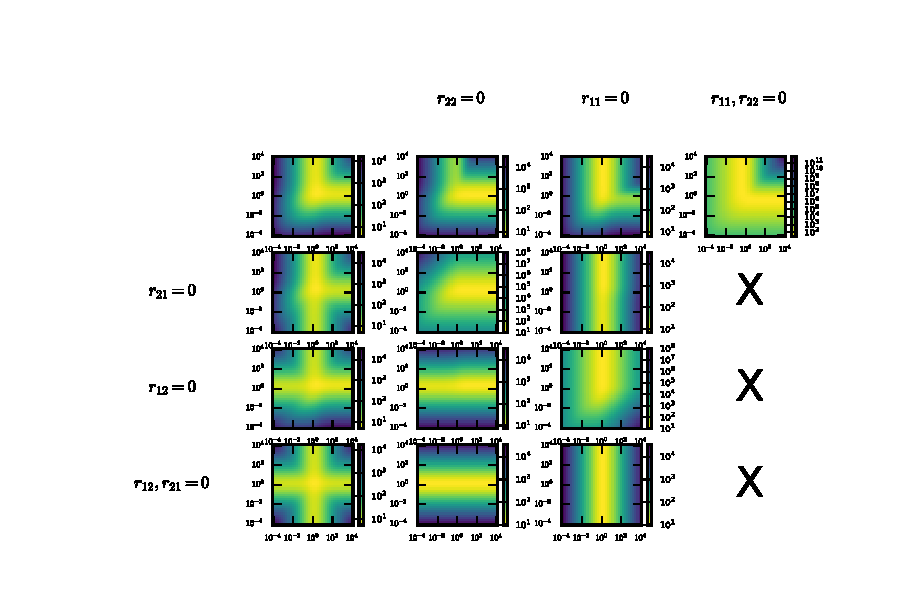
\includegraphics[width=\textwidth]{images/muslimit_allcombinations.pdf}
	\caption{Overview of the behaviour of $\omega$ at the service rate limits, for all combinations of transition probabilities.}
	\label{fig:all_combinations_mus_limits}
\end{center}
\end{figure}

The next few subsections will describe the behaviour of each combination in more detail. Below are three generic explanations that will be used to explain the behaviour of $\omega$ in the limit, as the service rate approaches $0$ and $\infty$.

\textbf{Explanation 1}: Consider Node $i$ with service rate $\mu_i$. As the service rate approaches $\infty$, the service time and Node $i$ approaches $0$. This implies that the time spent at that node approaches $0$, and no queue builds up. In that case, the time until a blockage approaches $\infty$, and so the time to a deadlock involving Node $i$ approaches $\infty$.

\textbf{Explanation 2}: Consider Node $i$ with service rate $\mu_i$. As the service rate approaches $0$, the service tmie at Node $i$ approaches $\infty$. This implies that no customer ever leaves Node $i$, and so the time until a blockage approaches $\infty$. Therefore the time until a deadlock involving Node $i$ approaches $\infty$.

\textbf{Explanation 3}: Consider Node $i$ with service rate $\mu_i$, and Node $j$ with service rate $\mu_j$. It was shown in \textbf{Explanation 2} that as $\mu_i$ approaches $0$ then no customer ever leaves Node $i$. Therefore a queue may build up, and a customer from Node $j$ may get blocked to Node $i$. This customer will only get unblocked and leave Node $j$ if a customer leaves Node $i$, which won't happen. Therefore no more customers will leave Node $j$, and by \textbf{Explanation 2} the time until a deadlock involving Node $j$ approaches $\infty$.

\textbf{Explanation 4}: Consider Node $i$, with outgoing transition probabilities $r_{ii}$ and $r_{ij}$. If $r_{ii} = r_{ij} = 0$, then all customers leaving Node $i$ also leave the system, and no blockages can occur at that node. Therefore the time to deadlock approaches $\infty$.

All of the situations described in the next subsections can be explained using a combination of these explanations.


\subsection{Service Rate Limits, $r_{12}, r_{21} = 0$, $r_{11}, r_{22} \neq 0$}\label{sec:r11r22}

When $r_{12} = 0$ and $r_{21} = 0$, the system is equivalent to two separate one node systems. Customers cannot transfer from one node to the other. The time to deadlock of the whole system is simply the minimum time to deadlock of both these separate one node systems. From the heatmap in Figure~\ref{fig:r11r22}, the following behaviour is observed at following limits:

\begin{figure}[htbp!]
	\begin{center}
		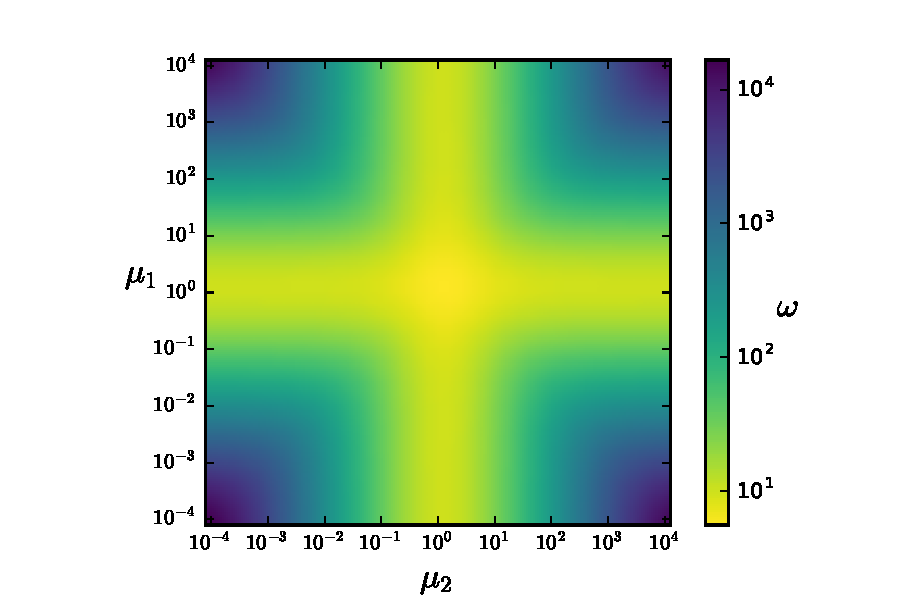
\includegraphics[width=0.45\textwidth]{images/r11r22.pdf}
	\end{center}
	\caption{Heatmap showing the time to deadlock, $\omega$, of the $\Omega$ system with $r_{12}, r_{21} = 0$.}
	\label{fig:r11r22}
\end{figure}

\begin{equation}\label{eqn:r12r21_infinf}
\lim_{\mu_1 \to \infty} \lim_{\mu_2 \to \infty} \omega = \infty
\end{equation}

\begin{equation}\label{eqn:r12r21_inf0}
\lim_{\mu_1 \to \infty} \lim_{\mu_2 \to 0} \omega = \infty
\end{equation}

\begin{equation}\label{eqn:r12r21_0inf}
\lim_{\mu_1 \to 0} \lim_{\mu_2 \to \infty} \omega = \infty
\end{equation}

\begin{equation}\label{eqn:r12r21_00}
\lim_{\mu_1 \to 0} \lim_{\mu_2 \to 0} \omega = \infty
\end{equation}

As mentioned before, this system is equivalent to two separate one node systems. Consider one of these systems $i$. Explanations 1 and 2 describe the limiting behaviour of this one node system. Now consider both separate nodes together. The time to deadlock of the system is the minimum time to deadlock of both nodes, and so in order to get an overall divergent time to deadlock, both nodes require divergent times to deadlock. Hence the behaviour described in Equations~\ref{eqn:r12r21_infinf}, \ref{eqn:r12r21_inf0}, \ref{eqn:r12r21_0inf}, \ref{eqn:r12r21_00}, and in Figure~\ref{fig:r11r22}.



\subsection{Service Rate Limits, $r_{ij}, r_{ji}, r_{ii} = 0$, $r_{jj} \neq 0$}\label{sec:rjj}

First consider the case when $i = 1$ and $j = 2$.
When $r_{12} = 0$, $r_{21} = 0$ and $r_{11} = 0$, the system is equivalent to two separate one node systems, however due to Explanation 4 Node 1 cannot reach deadlock. Customers cannot transfer from one node to the other. The time to deadlock of the whole system is simply time to deadlock of the one node system with feedback loop at Node 2. From the heatmaps in Figure~\ref{fig:rjj}the following behaviour is observed at following limits:

\begin{figure}[htbp!]
	\begin{center}
	  \begin{subfigure}{0.45\textwidth}
		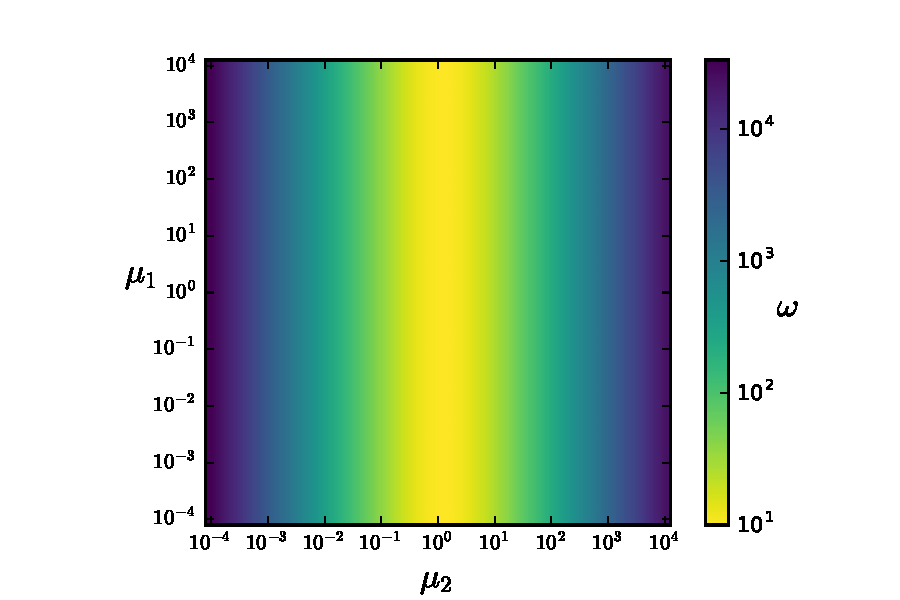
\includegraphics[width=\textwidth]{images/r22.pdf}
		\caption{When $i = 1$ and $j = 2$.}
	  \end{subfigure}
	  \begin{subfigure}{0.45\textwidth}
		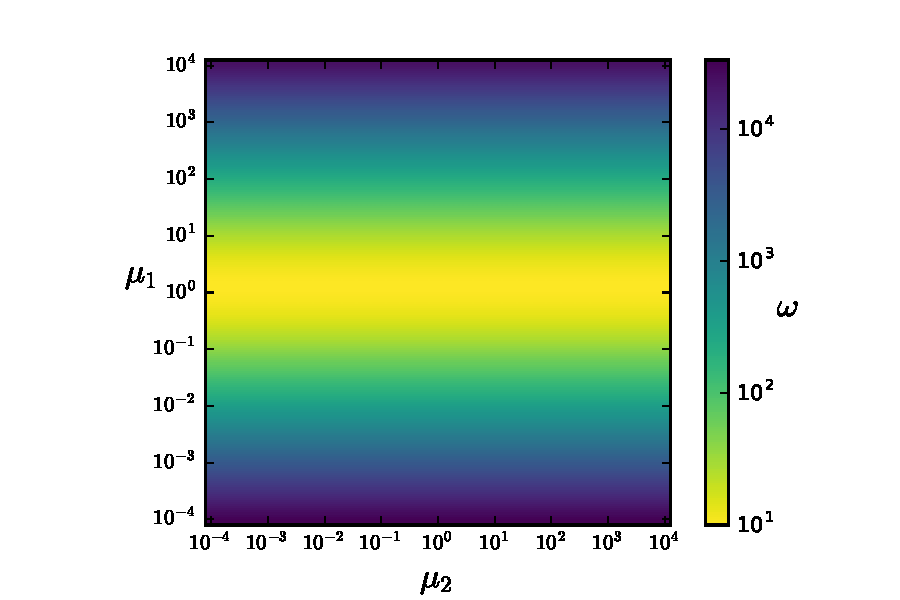
\includegraphics[width=\textwidth]{images/r11.pdf}
		\caption{When $i = 2$ and $j = 1$.}
	  \end{subfigure}
	\end{center}
	\caption{Heatmaps showing the time to deadlock of the $\Omega$ system where $r_{ij}, r_{ji}, r_{ii} = 0$.}
	\label{fig:rjj}
\end{figure}

\begin{equation}\label{eqn:r12r21r11_inf}
\lim_{\mu_2 \to \infty} \omega = \infty
\end{equation}

\begin{equation}\label{eqn:r12r21r11_0}
\lim_{\mu_2 \to 0} \omega = \infty
\end{equation}

Behaviour described in Equations~\ref{eqn:r12r21r11_inf} and \ref{eqn:r12r21r11_0}, and in Figure~\ref{fig:rjj}, in can be explained using Explanations 1 and 2.
Now consider the case where $i = 2$ and $j = 1$.
This system is the mirror of the system described above, and so by the same logic we find the following limits intuitive:

\begin{equation}\label{eqn:r12r21r22_inf}
\lim_{\mu_1 \to \infty} \omega = \infty
\end{equation}

\begin{equation}\label{eqn:r12r21r22_0}
\lim_{\mu_1 \to 0} \omega = \infty
\end{equation}

where $\mu_2$  has no effect on the time until deadlock $\omega$.


\subsection{Service Rate Limits, $r_{ji}, r_{ii} = 0$, $r_{ij}, r_{jj} \neq 0$}\label{sec:rijrjj}

First consider the case when $i = 1$ and $j = 2$.
When $r_{21} = 0$ and $r_{11} = 0$, only the deadlock involving Node 2 only can be reached. From the heatmaps in Figure~\ref{fig:rijrjj} the following behaviour is observed at following limits:

\begin{figure}[htbp!]
	\begin{center}
	  \begin{subfigure}{0.45\textwidth}
		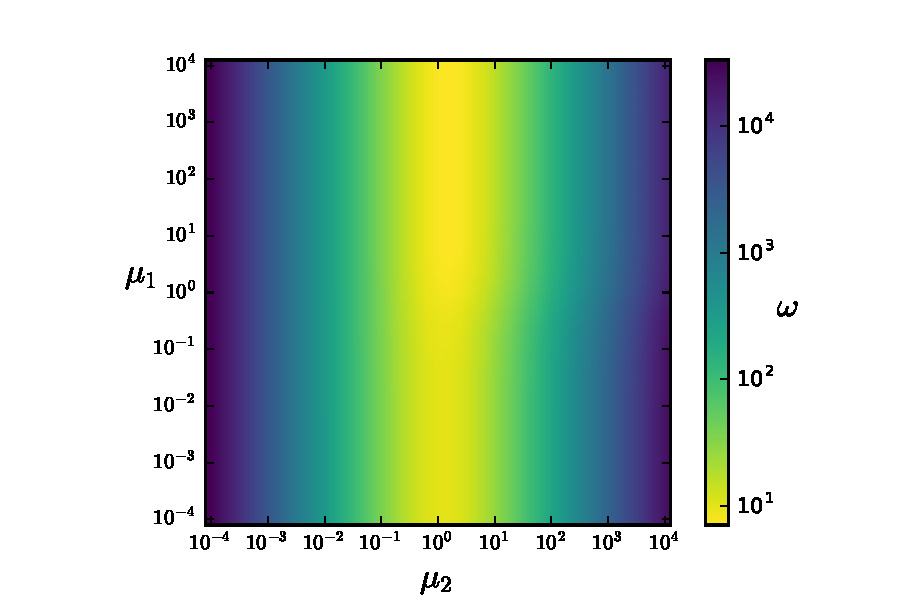
\includegraphics[width=\textwidth]{images/r12r22.pdf}
		\caption{When $i = 1$ and $j = 2$.}
	  \end{subfigure}
	  \begin{subfigure}{0.45\textwidth}
		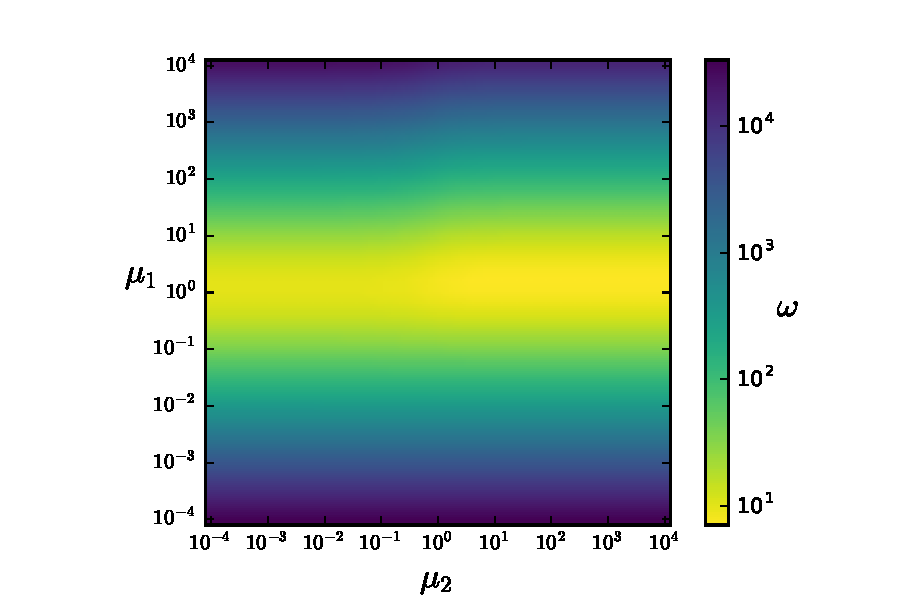
\includegraphics[width=\textwidth]{images/r11r21.pdf}
		\caption{When $i = 2$ and $j = 1$.}
	  \end{subfigure}
	\end{center}
	\caption{Heatmaps showing the time to deadlock of the $\Omega$ system where $r_{ji}, r_{ii} = 0$.}
	\label{fig:rijrjj}
\end{figure}

\begin{equation}\label{eqn:r12r22_inf}
\lim_{\mu_2 \to \infty} \omega = \infty
\end{equation}

\begin{equation}\label{eqn:r12r22_0}
\lim_{\mu_2 \to 0} \omega = \infty
\end{equation}

These limits, shown in Equations~\ref{eqn:r12r22_inf} and \ref{eqn:r12r22_0}, can be explained using Explanations 1 and 2.
In these systems however, the service rate $\mu_1$ does have an effect on the time until deadlock, but not at the limits. Here increasing $\mu_1$ simply contributes towards Node 2 having a greater effective arrival rate, increasing the time until deadlock slightly.

Now consider the case where $i = 2$ and $j = 1$.
This system is the mirror of the system described above, and so by the same logic we find the following limits intuitive:

\begin{equation}\label{eqn:r11r21_inf}
\lim_{\mu_1 \to \infty} \omega = \infty
\end{equation}

\begin{equation}\label{eqn:r11r21_0}
\lim_{\mu_1 \to 0} \omega = \infty
\end{equation}


\subsection{Service Rate Limits, $r_{12}, r_{21}, r_{11}, r_{22} \neq 0$}\label{sec:r11r12r21r22}

When no transition probability is set to zero, then we get the original $\Omega$ system.
From the heatmaps shown in Figure~\ref{fig:r11r12r21r22} the following behaviour is observed at following limits:

\begin{figure}[htbp!]
	\begin{center}
		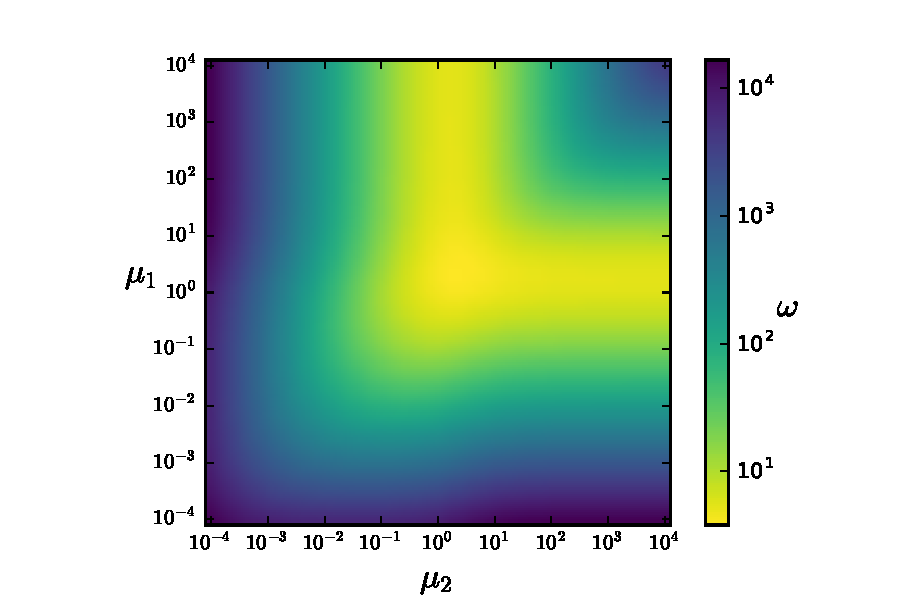
\includegraphics[width=0.45\textwidth]{images/r11r12r21r22.pdf}
	\end{center}
	\caption{Heatmap showing the time to deadlock, $\omega$, of the $\Omega$ system with $r_{12}, r_{21}, r_{11}, r_{22} = 0$.}
	\label{fig:r11r12r21r22}
\end{figure}

\begin{equation}\label{eqn:all_infinf}
\lim_{\mu_1 \to \infty} \lim_{\mu_2 \to \infty} \omega = \infty
\end{equation}

\begin{equation}\label{eqn:all_0_}
\lim_{\mu_1 \to 0} \omega = \infty
\end{equation}

\begin{equation}\label{eqn:all__0}
\lim_{\mu_2 \to 0} \omega = \infty
\end{equation}

As both $\mu_1$ and $\mu_2$ approach infinity, we see in Equation~\ref{eqn:all_infinf} that the time to deadlock diverges to $\infty$. This is intuitive using Explanation 1. Explanations 2 and 3 explain the limits as the service rates here approach $0$.


\subsection{Service Rate Limits, $r_{ij} = 0$, $r_{ji}, r_{ii}, r_{jj} \neq 0$}\label{sec:riirjirjj}

First consider the case when $i = 1$ and $j = 2$.
The system when only $r_{12} = 0$ is a cross between the behaviour we see in the systems described in Sections~\ref{sec:r11r22} and \ref{sec:r11r12r21r22}. From the heatmaps shown in Figure~\ref{fig:riirjirjj} the following behaviour is observed at following limits:

\begin{figure}[htbp!]
	\begin{center}
	  \begin{subfigure}{0.45\textwidth}
		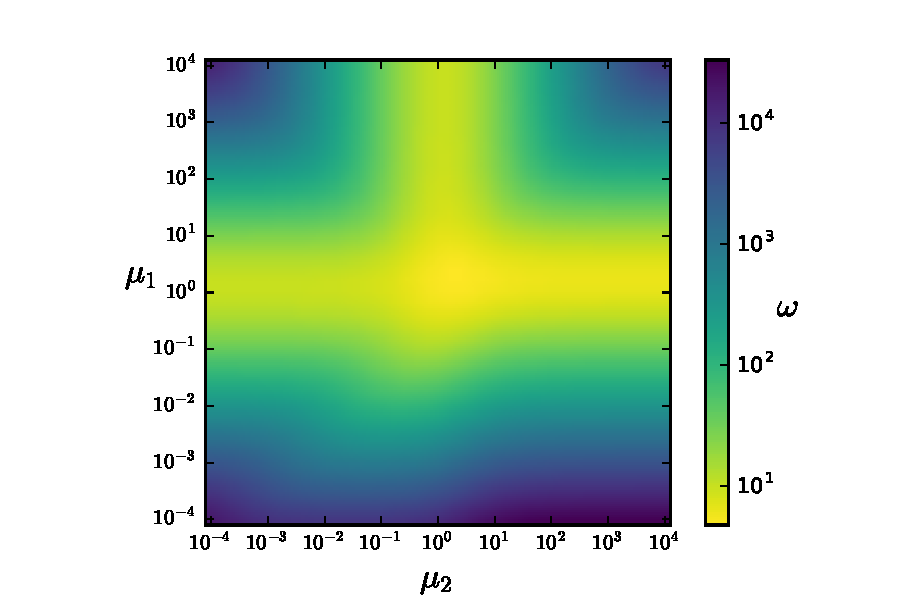
\includegraphics[width=\textwidth]{images/r11r21r22.pdf}
		\caption{When $i = 1$ and $j = 2$.}
	  \end{subfigure}
	  \begin{subfigure}{0.45\textwidth}
		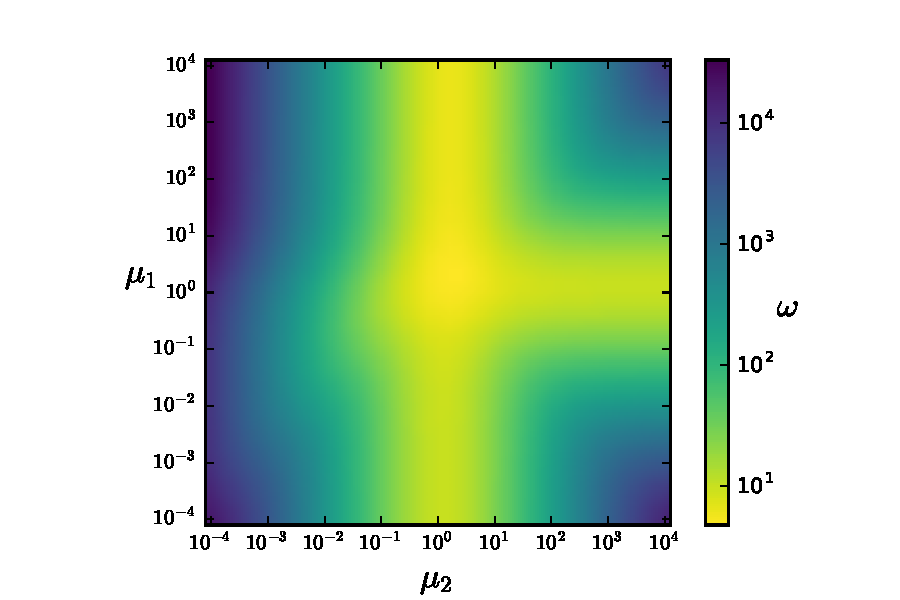
\includegraphics[width=\textwidth]{images/r11r12r22.pdf}
		\caption{When $i = 2$ and $j = 1$.}
	  \end{subfigure}
	\end{center}
	\caption{Heatmap showing the time to deadlock, $\omega$, of the $\Omega$ system with $r_{ij} = 0$.}
	\label{fig:riirjirjj}
\end{figure}

\begin{equation}\label{eqn:r12_infinf}
\lim_{\mu_1 \to \infty} \lim_{\mu_2 \to \infty} \omega = \infty
\end{equation}

\begin{equation}\label{eqn:r12_inf0}
\lim_{\mu_1 \to \infty} \lim_{\mu_2 \to 0} \omega = \infty
\end{equation}

\begin{equation}\label{eqn:r12_0_}
\lim_{\mu_1 \to 0} \omega = \infty
\end{equation}

As both $\mu_1$ and $\mu_2$ approach infinity, we see in Equation~\ref{eqn:r12_infinf} that the time to deadlock diverges to $\infty$, due to Explanation 1.
As $\mu_1$ approaches infinity and $\mu_2$ approaches $0$, then the time to deadlock diverges to $\infty$, due to Explanations 1 and 2.
Finally as $\mu_1$ approaches $0$, then the time to deadlock diverges to $\infty$, due to Explanation 3.

Now consider the case where $i = 2$ and $j = 1$.
This system is the mirror of the system described above, and so by the same logic we find the following limits intuitive:

\begin{equation}\label{eqn:r21_infinf}
\lim_{\mu_1 \to \infty} \lim_{\mu_2 \to \infty} \omega = \infty
\end{equation}

\begin{equation}\label{eqn:r21_inf0}
\lim_{\mu_1 \to 0} \lim_{\mu_2 \to \infty} \omega = \infty
\end{equation}

\begin{equation}\label{eqn:r21_0_}
\lim_{\mu_2 \to 0} \omega = \infty
\end{equation}


\subsection{Service Rate Limits, $r_{ii} = 0$, $r_{ij}, r_{ji}, r_{jj} \neq 0$}\label{sec:rijrjirjj}

First consider the case when $i = 1$ and $j = 2$. There are only two deadlocks that can be reached, both involving Node 2.
From the heatmaps in Figure~\ref{fig:rijrjirjj} the following behaviour is observed at following limits:

\begin{figure}[htbp!]
	\begin{center}
	  \begin{subfigure}{0.45\textwidth}
		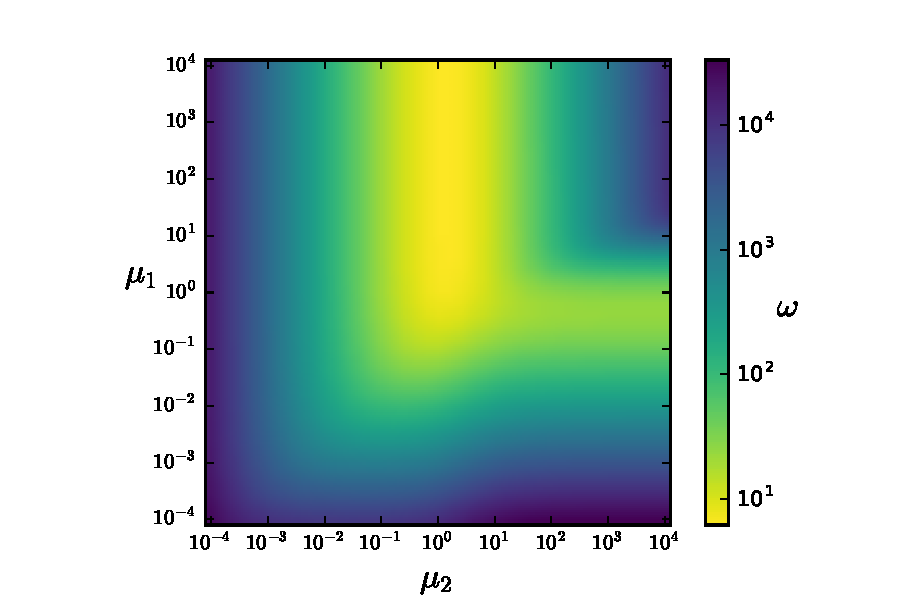
\includegraphics[width=\textwidth]{images/r12r21r22.pdf}
		\caption{When $i = 1$ and $j = 2$.}
	  \end{subfigure}
	  \begin{subfigure}{0.45\textwidth}
		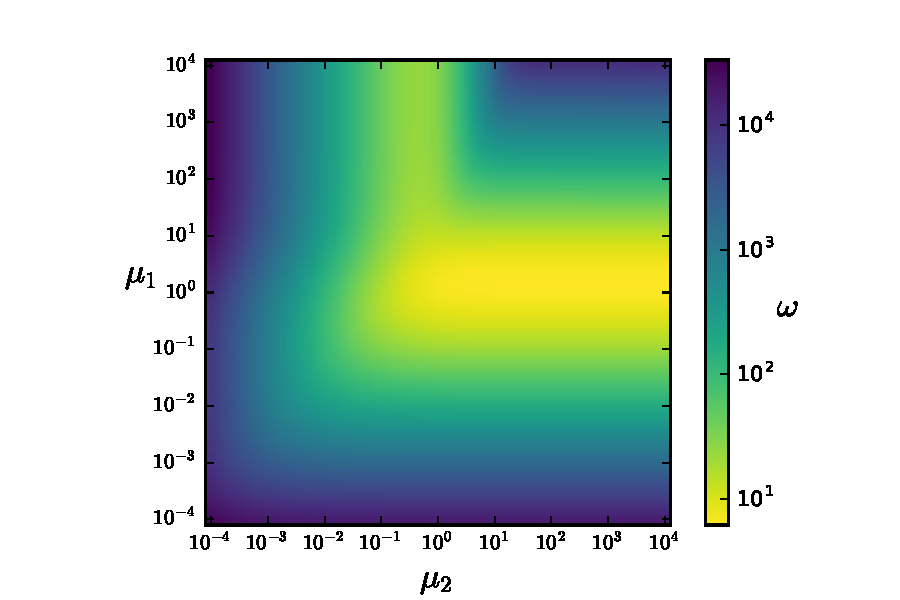
\includegraphics[width=\textwidth]{images/r11r12r21.pdf}
		\caption{When $i = 2$ and $j = 1$.}
	  \end{subfigure}
	\end{center}
	\caption{Heatmaps showing the time to deadlock of the $\Omega$ system where $r_{ii} = 0$.}
	\label{fig:rijrjirjj}
\end{figure}

\begin{equation}\label{eqn:r11_inf}
\lim_{\mu_1 \to \infty} \lim_{\mu_2 \to \infty} \omega = \infty
\end{equation}

\begin{equation}\label{eqn:r11__0}
\lim_{\mu_2 \to 0} \omega = \infty
\end{equation}

\begin{equation}\label{eqn:r11_0_}
\lim_{\mu_1 \to 0} \omega = \infty
\end{equation}

As both $\mu_1$ and $\mu_2$ approach infinity the time until deadlock approaches infinity, as shown in Equation~\ref{eqn:r11_inf}. This is intuitive due to Explanation 1.
As $\mu_2$ and $\mu_1$ approach $0$ the time until a deadlock approaches $\infty$, this is due to Explanations 2 and 3.


Now consider the case where $i = 2$ and $j = 1$.
This system is the mirror of the system described above, and so by the same explanations the following limits exist:

\begin{equation}\label{eqn:r22_inf}
\lim_{\mu_1 \to \infty} \lim_{\mu_2 \to \infty} \omega = \infty
\end{equation}

\begin{equation}\label{eqn:r22__0}
\lim_{\mu_2 \to 0} \omega = \infty
\end{equation}

\begin{equation}\label{eqn:r22_0_}
\lim_{\mu_1 \to 0} \omega = \infty
\end{equation}


\subsection{Service Rate Limits, $r_{ii}, r_{ij} = 0$, $r_{ji}, r_{jj} \neq 0$}\label{rjirjj}

First consider the case where $i = 1$ and $j = 2$.
In this case, $r_{11}, r_{12} = 0$, and so by Explanation 4 only one deadlock is possible, the deadlock involving Node 2 only.

From the heatmaps shown in Figure~\ref{fig:rjirjj}, the following behaviour is observed at following limits:

\begin{figure}[htbp!]
	\begin{center}
	  \begin{subfigure}{0.45\textwidth}
		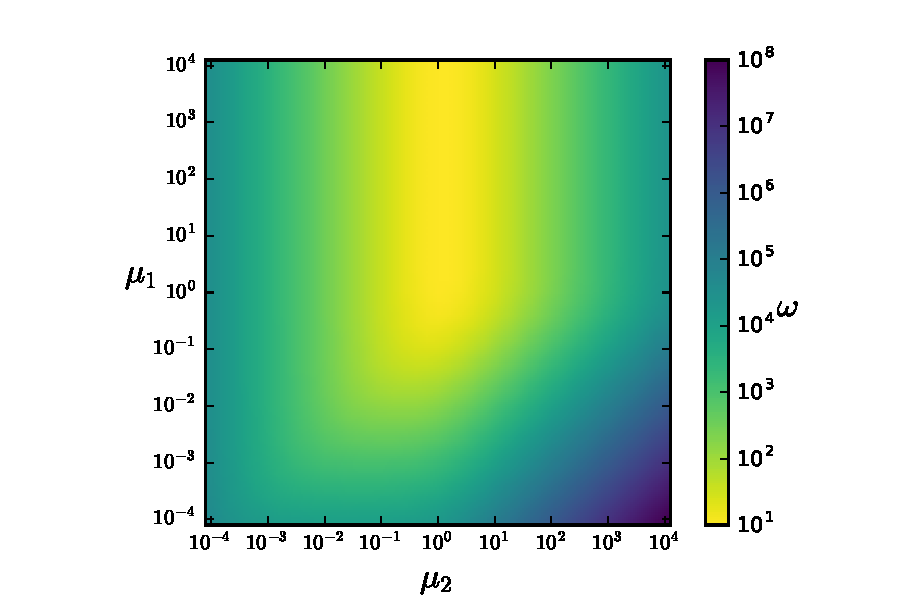
\includegraphics[width=\textwidth]{images/r21r22.pdf}
		\caption{When $i = 1$ and $j = 2$.}
	  \end{subfigure}
	  \begin{subfigure}{0.45\textwidth}
		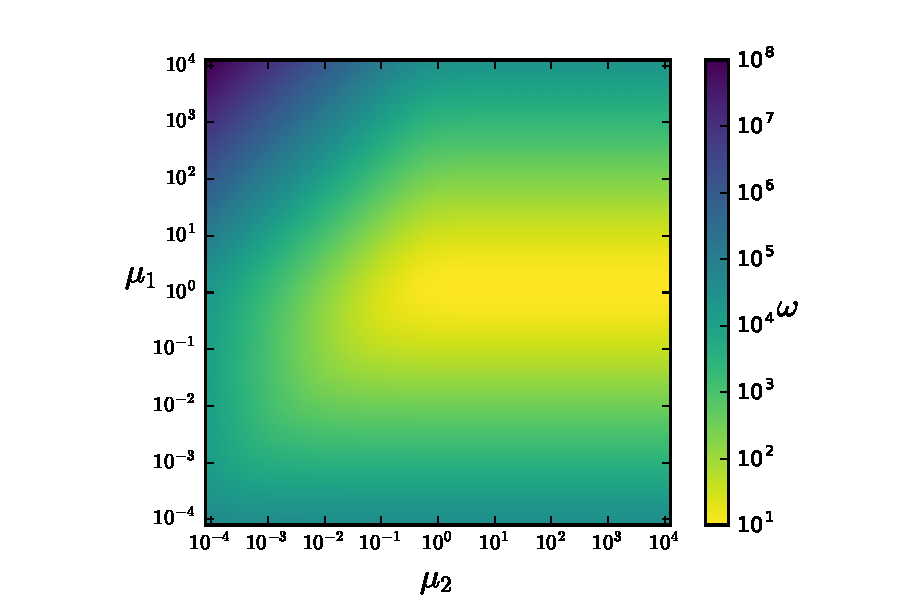
\includegraphics[width=\textwidth]{images/r11r12.pdf}
		\caption{When $i = 2$ and $j = 1$.}
	  \end{subfigure}
	\end{center}
	\caption{Heatmaps showing the time to deadlock of the $\Omega$ system where $r_{ii}, r_{ij} = 0$.}
	\label{fig:rjirjj}
\end{figure}


\begin{equation}\label{eqn:r21r22_0_}
\lim_{\mu_1 \to 0} \omega = \infty
\end{equation}

\begin{equation}\label{eqn:r21r22__inf}
\lim_{\mu_2 \to \infty} \omega = \infty
\end{equation}

\begin{equation}\label{eqn:r21rr22__0}
\lim_{\mu_2 \to 0} \omega = \infty
\end{equation}

As $\mu_2$ approaches either $\infty$ or $0$, the time until deadlock approaches $\infty$. This is due to Explanations 2 and 3.
As $\mu_1$ approaches $0$ Explanation 3 tells us that the time to deadlock involving Node 2 approaches $\infty$. As only deadlocks involving Node 2 can occur, then the time to deadlock of the system also approaches $\infty$.


Now consider the case where $i = 2$ and $j = 1$.
This system is the mirror of the system described above, and so by the same explanations the following limits exist:

\begin{equation}\label{eqn:r21r22_0_}
\lim_{\mu_1 \to 0} \omega = \infty
\end{equation}

\begin{equation}\label{eqn:r21r22__inf}
\lim_{\mu_1 \to \infty} \omega = \infty
\end{equation}

\begin{equation}\label{eqn:r21rr22__0}
\lim_{\mu_2 \to 0} \omega = \infty
\end{equation}


\subsection{Service Rate Limits, $r_{ii}, r_{jj} = 0$, $r_{ij}, r_{ji} \neq 0$}\label{sec:rijrji}

This system is equivalent to an $\Omega_2$ system, where only one deadlock can be reached.
From the heatmaps shown in Figure~\ref{fig:rijrji}, the following behaviour is observed at following limits:

\begin{figure}[htbp!]
	\begin{center}
		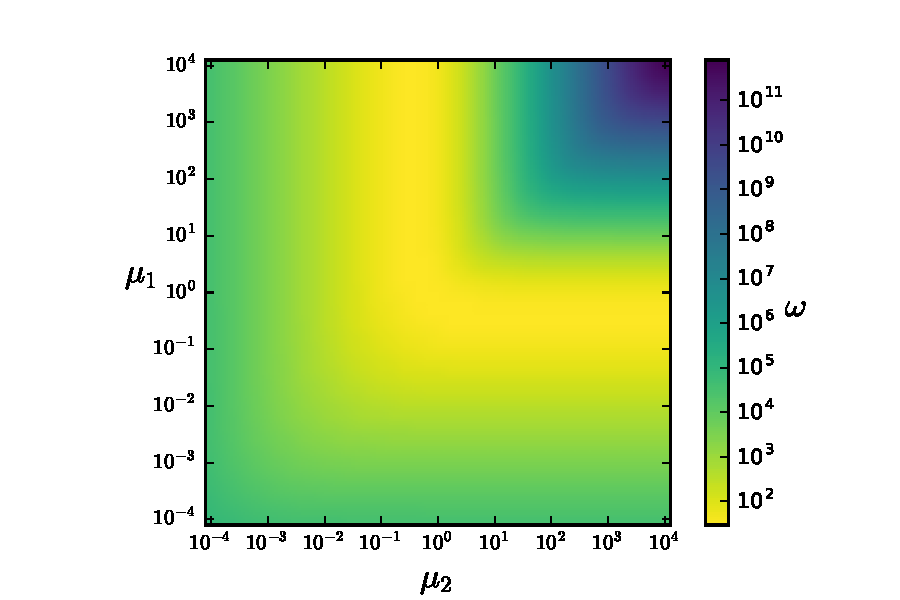
\includegraphics[width=0.45\textwidth]{images/r12r21.pdf}
	\end{center}
	\caption{Heatmap showing the time to deadlock, $\omega$, of the $\Omega$ system with $r_{12}, r_{21} = 0$.}
	\label{fig:rijrji}
\end{figure}

\begin{equation}\label{eqn:all_infinf}
\lim_{\mu_1 \to \infty} \lim_{\mu_2 \to \infty} \omega = \infty
\end{equation}

\begin{equation}\label{eqn:all_0_}
\lim_{\mu_1 \to 0} \omega = \infty
\end{equation}

\begin{equation}\label{eqn:all__0}
\lim_{\mu_2 \to 0} \omega = \infty
\end{equation}

Explanation 1 can be used for the limit shown in Equation~\ref{eqn:all_infinf}, and Explanations 2 and 3 can be used for the limit shown in Equations~\ref{eqn:all_0_} and \ref{eqn:all__0}.


\end{document}